\chapter{Monte Carlo Integration}\label{ch:monte-carlo}
For a one-dimensional integral, the simplest method is to compute the sum of the area of regions over the domain. If the regions are uniformly spaced, the approximation of the integral $I$ is:

\begin{figure}
\sidecaption
	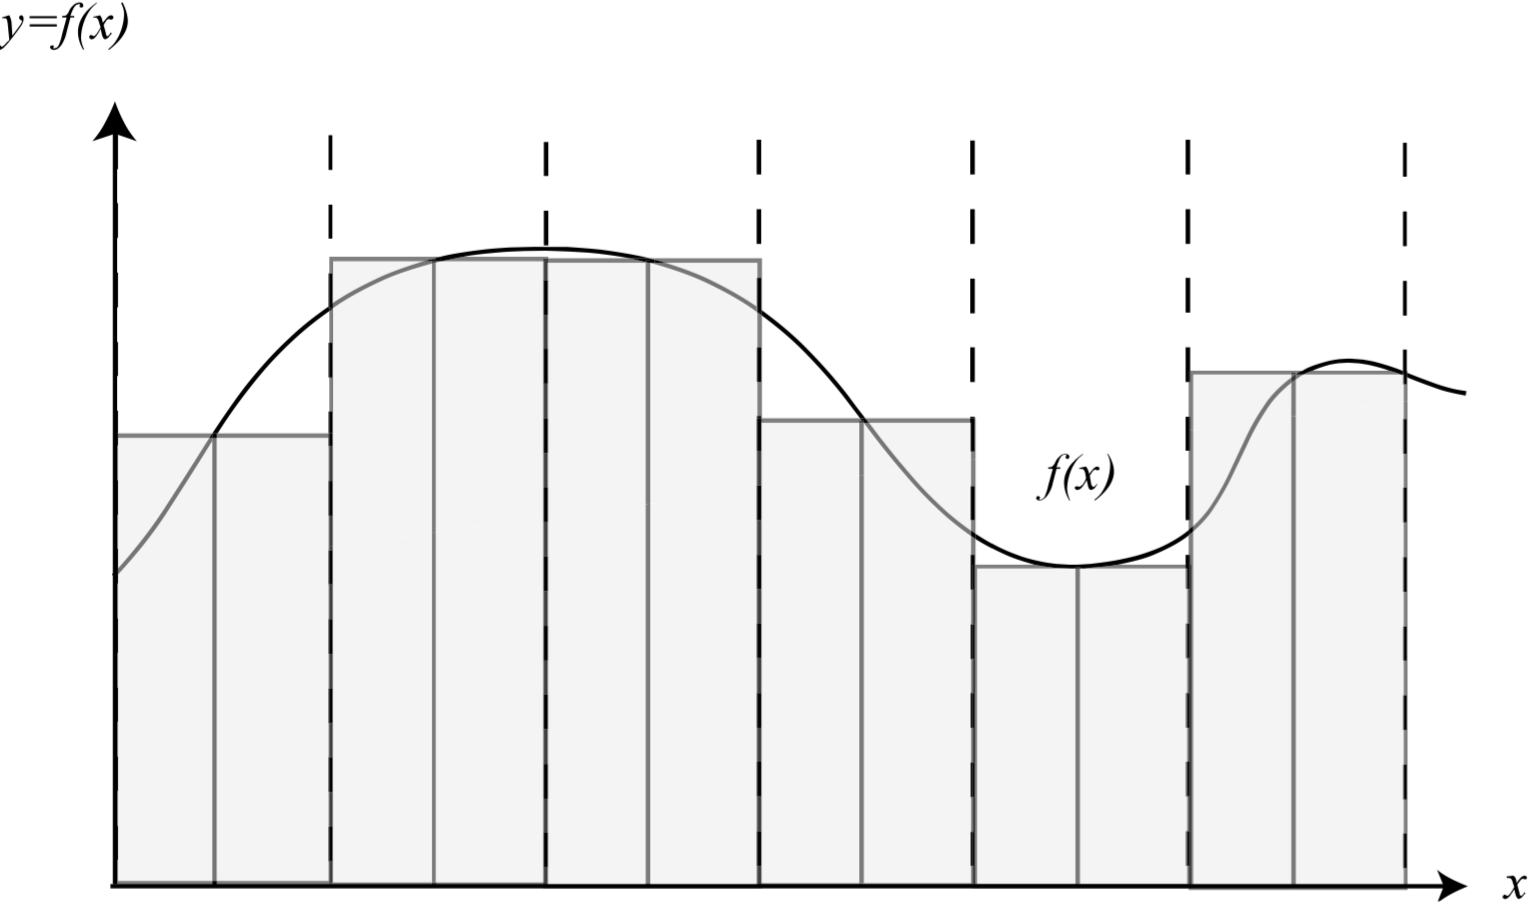
\includegraphics[width=0.65\textwidth]{graphics/gi/mc-1}
	\caption{Deterministic one-dimensional integration.}
	\label{f:quadrature-rules}
\end{figure} 

\begin{equation}
	\begin{aligned}
		I&=\int_{a}^{b}f(x)dx \\
		&\approx \sum_{i=1}^{N}f(x_i)\frac{(b-a)}{N}
	\end{aligned}
\end{equation}

where $f(x_i)$ is the middle point of the interval. Such method is called \textit{quadrature rules} and can be seen in figure \ref{f:quadrature-rules}.

Extending this deterministic quadrature rules to a $d-$dimensional integral would require $N^d$ samples. Obviously, it's not applicable to multidimensional integrals. There are some methods for multidimensional integrals\footnote{\url{https://en.wikipedia.org/wiki/Numerical_integration\#Multidimensional\_integrals}}, the most used method in computer graphics is Monte Carlo integration. Monte Carlo method has many applications, one of the most important of which is high dimensional integrals.

Monte Carlo method is quiet simple: it simulates an experimental measuring process with sampling and averaging. In this section we discuss Monte Carlo integration by four questions: What is Monte Carlo integration in section \ref{sec:Monte-Carlo-Integration}? How to sampling variables in section \ref{sec:Sampling-Random-Variables}? And since Monte Carlo method is an approximation of the real solution of the integral, the last section \ref{sec:Variance-Reduction} will introduce some methods to reduce the variances.

This section is a brief introduction of Monte Carlo method. For more details, \cite[-30mm]{a:EfficientMonteCarloMethodsforLightTransportinScatteringMedia} is a good start; \cite[-15mm]{b:AdvancedGlobalIllumination} includes a through discussion about Monte Carlo method and how it is used in global illumination; And \cite[-5mm]{b:pbrt} details how implement Monte Carlo integration in the code.



\section{Probability Background}
The Monte Carlo integration involves sampling an appropriate random variable and averaging the estimates obtained from the sample. So we need to review the probability theory, from which We then can derive the magical, simple and powerful Monte Carlo estimator for integral. 

\subsection{Random Variables}
A \textit{random variable X} is a function that maps outcomes of a random process to a numbers. A random variable can take a set of possible different values, each with an associated probability, which described by the \textit{probability density function} (PDF), $p$. 

A random variable can be discrete, such as in the Dice game, every roll event is mapped to a random variable $x_i$, where $X=\{1,2,3,4,5,6\}$, and every random variable has a probability $p_i=1/6$, or continuous. For a discrete random variable:

\begin{equation}
	\begin{aligned}
		0\leq &p_i \leq 1 \\
		\sum_i &p_i=1
	\end{aligned}
\end{equation}

For a continuous random variable $x$, a probability density function  $p(x)$ is defined such that the probability that the variable takes a value $x$ in the interval $[x,x+dx]$ equals $p(x)dx$. A \textit{cumulative distribution function (CDF)} provides a more intuitive definition of probabilities for continuous variables. The CDF for a random variable $x$ is defined as follows:

\begin{equation}
	P(y)=Pr(x\leq y)=\int_{-\infty}^{y}p(x)dx
\end{equation}

The CDF gives the probability with which an event occurs with an outcome whose value is less than or equal to the value $y$. The PDF $p(x)$ for continuous random variable has the following properties:

\begin{equation}
	\begin{aligned}
		\forall x: p(x)&\geq 0;\\
		\int_{-\infty}^{+\infty}p(x)dx&=1;\\
		p(x)&=\frac{dP(x)}{dx}
	\end{aligned}
\end{equation}

The probability that x will take on a value in some interval $[a,b]$ is:

\begin{equation}
	\begin{aligned}
		Pr(a\leq x\leq b)&=Pr(x\leq b)-Pr(x\leq a)\\
		&=P(b)-P(a)=\int_{a}^{b}p(z)dz
	\end{aligned}
\end{equation} 



\subsection{Expected Value}
For a discrete random variable with $n$ possible outcomes, the \textit{expected value}, or \textit{mean}, of the random variable is:

\begin{equation}
	E(x)=\sum_{i=1}^{n}p_i x_i
\end{equation} 

For the case of a fair dice, the expected value of the dice throws is:

\begin{equation*}
	\begin{aligned}
		E(x_{die})&=\sum_{i=1}^{6}p_i x_i\\
		&=\sum_{i=1}^{6}\frac{1}{6}x_i =\frac{1}{6}(1+2+3+4+5+6)\\
		&=3.5
	\end{aligned}
\end{equation*}

Similar, the expected value of a continuous random variable $x$ is:

\begin{equation}
	E(x)=\int_{-\infty}^{+\infty}xp(x)dx
\end{equation}


\subsection{Variance}
The \textit{variance} $\sigma^2$, denoted as $V\{X\}$ is a measure of the deviation of the outcomes from the expected value of the random variable. The \textit{standard deviation} $\sigma$ is the square root of the variance. The variance is defined as:

\begin{equation}
	\sigma^2=E[(x-E[x])^2]=\sum_i (x_i-E[x])^2p_i
\end{equation}

for discrete random variables and:

\begin{equation}\label{e:discrete-variance}
	\sigma^2=E[(x-E[x])^2]=\int (x-E[x])^2 p(x)dx
\end{equation}

The variance has the following properties:
\begin{enumerate}
	\item For a random variance $C$, which is constant(i.e. the random variable equals $C$ with probability 1),
	\begin{equation}
		V\{C\}=0
	\end{equation}
	\item For a constant $C$ and random variable $X$,
	\begin{equation}
		V\{CX\}=C^2V\{X\}
	\end{equation}
	\item For independent random variables $X$ and $Y$,
	\begin{equation}
		V\{X+Y\}=V\{X\}+\{Y\}
	\end{equation}
\end{enumerate}


\subsection{Estimated Means}
Many problems involve sums of independent random variables $x_i$, where the variables share a common density $p$. Such variables are said to be \textit{independent identically distributed (IID)} random variables. When the sum is divided by the number of variables, we get an estimate of $E(x)$:

\begin{equation}
	E(x)\approx \frac{1}{N} \sum_{i=1}^{N}x_i
\end{equation}

As $N$ increases, the variance of this estimate decreases. We want $N$ to be large enough that we have confidence that the estimate is "close enough". However, there are no sure things in Monte Carlo; we just gain statistical confidence that our estimate is good. To be sure, we would have to have $n=\infty$. This confidence is expressed by \textit{Law of Large Number}:

\begin{equation}
	Pr\Bigg[ E(x)=\lim_{N \to \infty}\frac{1}{N}\sum_{i=1}^{N}x_i \Bigg]=1
\end{equation} 



\section{Monte Carlo Integration}\label{sec:Monte-Carlo-Integration}
Now we describe how Monte Carlo techniques can be used for the integration of arbitrary functions. Let us assume we have some function $g(x)$ defined over the domain $x\in S$. We would like to evaluate the integral:

\begin{equation}
	I=\int_{x\in S}g(x)d\mu
\end{equation}

As discussed earlier, given a function $f$ and a random variable $x\sim p$, we can approximate the expected value of $f(x)$ by a sum:

\begin{equation}\label{e:sum}
	E(f(x))=\int_{x\in S}f(x)p(x)d\mu\approx\frac{1}{N}\sum_{i=1}^{N}f(x_i)
\end{equation}

This result leads to the central idea of Monte Carlo evaluation of integrals. Because the expected value can be expressed as an integral, the integral is also approximated by the sum. The form of equation \ref{e:sum} is a bit awkward, we could usually like to approximate an integral of a single function $g$ rather than a product $fp$. We can get around this by substituting $g=fp$ as the integrand:

\begin{equation}
	\int_{x\in S}g(x)d\mu\approx\frac{1}{N}\sum_{i=1}^{N}\frac{g(x_i)}{p(x_i)}
\end{equation}

For this formula to be valid, $p$ must be positive where $g$ is nonzero. We denote the estimator as $\langle I\rangle$ and is:

\begin{equation}
	\langle I\rangle=\frac{1}{N}\sum_{i=1}^{N}\frac{g(x_i)}{p(x_i)}
\end{equation}

The expected value of this estimator is computed as follows:

\begin{equation}
	\begin{aligned}
		E[\langle I\rangle]&=E[\frac{1}{N}\sum_{i=1}^{N}\frac{g(x_i)}{p(x_i)}]\\
		&=\frac{1}{N}\sum_{i=1}^{N}E[\frac{g(x_i)}{p(x_i)}]\\
		&=\frac{1}{N}N\int \frac{g(x)}{p(x)}p(x)dx\\
		&=\int g(x)dx\\
		&=I
	\end{aligned}
\end{equation}

From equation \ref{e:discrete-variance}, we know that the variance of this estimator is:

\begin{equation}\label{e:variance}
	\sigma^2=\frac{1}{N}\int(\frac{g(x)}{p(x)}-I)^2p(x)dx
\end{equation}

Thus, as $N$ increases, the variance decreases linearly with $N$. The error in the estimator is proportional to the standard deviation $\sigma$; the standard deviation decreases as $\sqrt{N}$. This is a classic result of Monte Carlo methods. In fact one problem with Monte Carlo is the slow convergence of the estimator to the right solution; four times more samples are required to decrease the error of the Monte Carlo computation by half.

In a summary, Monte Carlo integration is a powerful, general technique that can handle arbitrary functions. A Monte Carlo computation consists of the following steps:

\begin{itemize}
	\item Sampling according to a probability distribution function.
	\item Evaluation of the function at that sample.
	\item Averaging these appropriately weighted sampled values.
\end{itemize}

In these steps, the most difficult work is how to sample random variables for a arbitrary function. The next section we will talk about random variable generation, and in section \ref{sec:Variance-Reduction}, we introduce some general method to reduce the variance.



\section{Sampling Random Variables}\label{sec:Sampling-Random-Variables}
In doing Monte Carlo calculation, it is required that random variables be drawn from distribution functions that define the stochastic process. The process of "sampling $X$ from $f(x)$" is therefore an essential technical matter.

First let's define what we mean by \textit{sampling}. Consider some space $\Omega_0$ and $x\in\Omega_0$, together with a probability distribution function $f(x)$, where

\begin{equation}
	\int_{\Omega_0}f(x)dx=1
\end{equation}

A sampling procedure is an algorithm that can produce a sequence of values of $X$ ("random variables") $X_1,X_2,...$ such that for any $\Omega\in\Omega_0$

\begin{equation}
	P\{X_k\in\Omega\}=\int_{\Omega}f(x)dx\leq 1
\end{equation}

It will be possible to do this only by already having a sequence of some basic random variables. In a computer program, a method random(u) can generate  uniformly distributed random variables(called \textit{pseudorandom numbers}), we denote these by $\xi_1,\xi_2,...$, which can be such basic random variables.



\subsection{The Inversion Method}
\begin{figure}
\sidecaption
	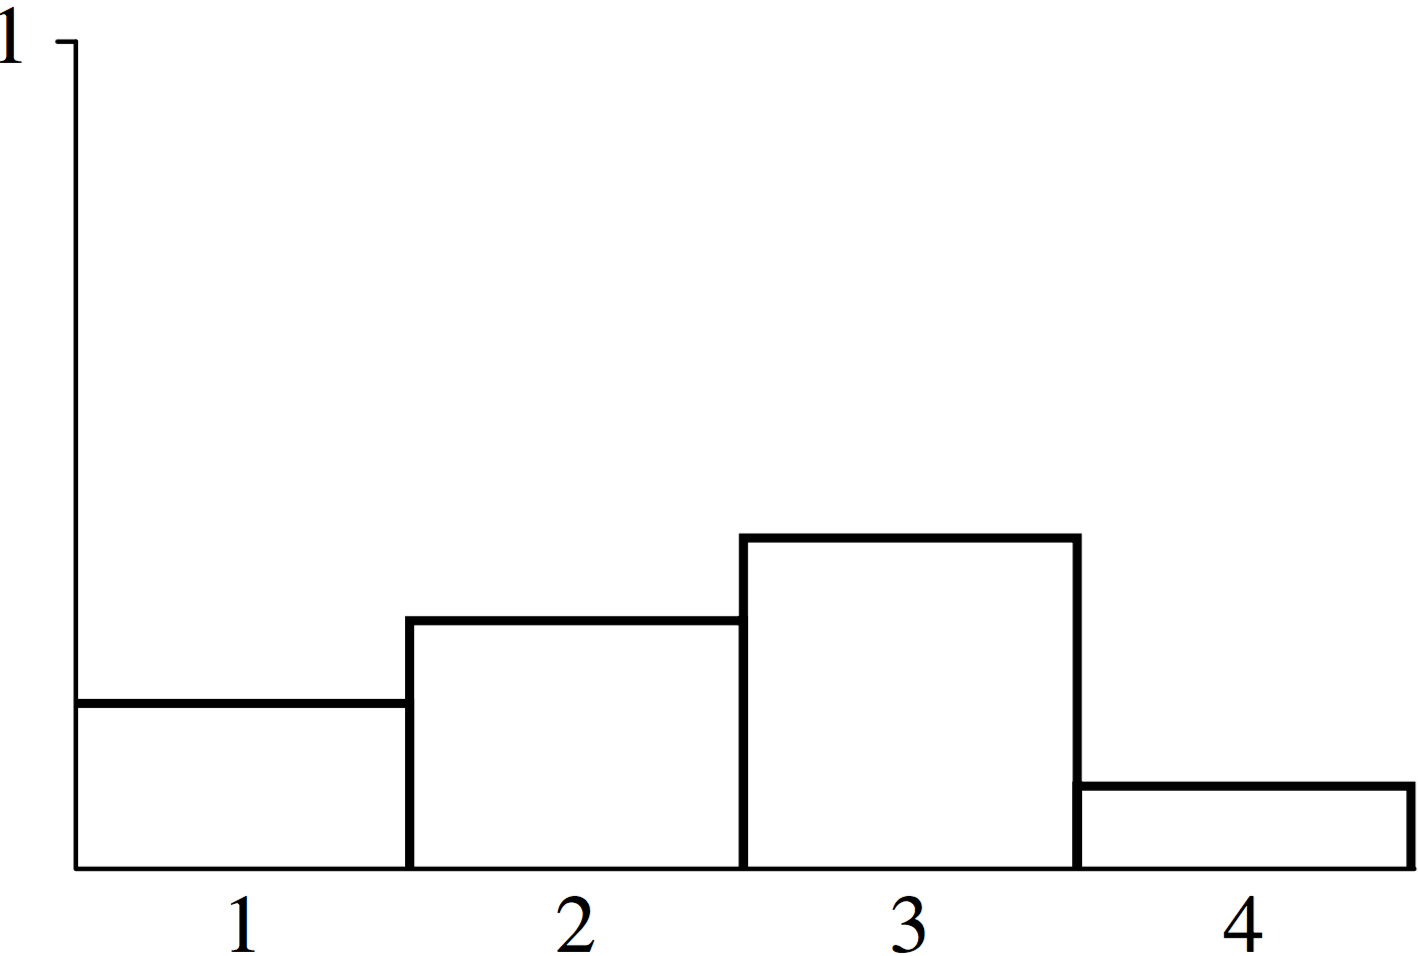
\includegraphics[width=0.65\textwidth]{graphics/gi/mc-3}
	\caption{A discrete PDF for four events each with a probability $p_i$.}
	\label{f:simple-pdf}
\end{figure}

The inversion method uses one or more uniform random variables, which produced from random(u) and maps them to random variables from the desired distribution. We explain this process with a simple discrete example with four possible outcomes. The probabilities of each of the four outcomes are given by $p_1,p_2,p_3$ and $p_4$ that $\sum_{i=1}^{4}p_i=1$, The corresponding PDF is shown in figure \ref{f:simple-pdf}.

In order to draw a sample from this distribution, we first find the CDF $P(x)$. In the continuous case, $P$ is the indefinite integral of $p$. In the discrete case, we can sum the $i$ $p$s as the value of $P(x_i)$, see figure \ref{f:simple-cdf}. Notice that the height of the rightmost bar must be one because of the requirement that all probabilities sum to one.

\begin{figure}
\sidecaption
	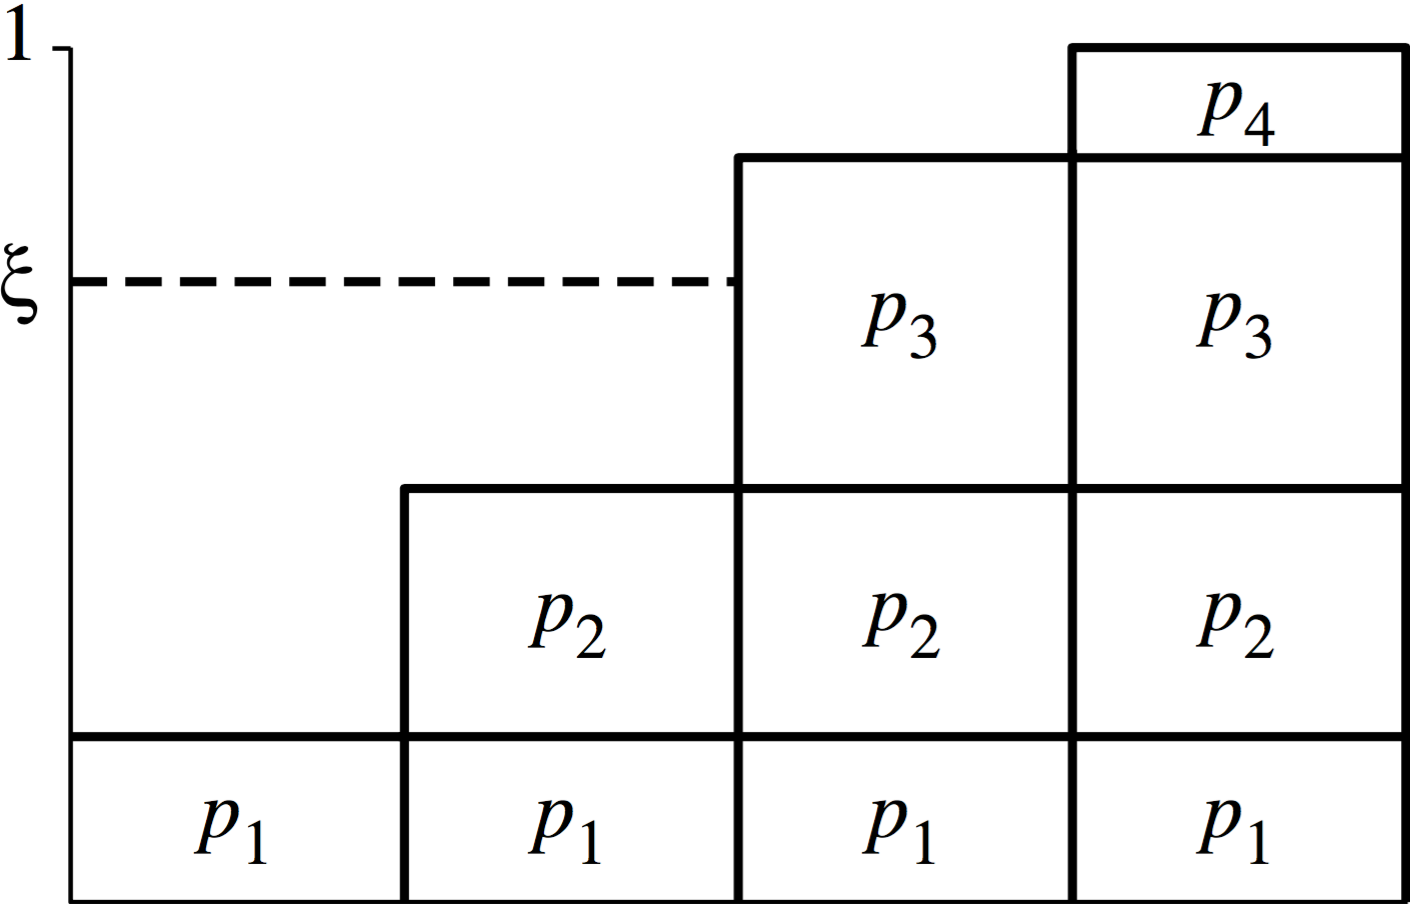
\includegraphics[width=0.65\textwidth]{graphics/gi/mc-4}
	\caption{To use the inversion method to draw a sample from the distribution described by the PDF in \ref{f:simple-pdf}, a canonical uniform random variable is plotted on the vertical axis. By construction, the horizontal extension of $\xi$ will intersect the box representing the $i$th outcome with probability $p_i$. If the corresponding event is chosen for a set of random variables $\xi$, then the resulting distribution of events will be distributed according to the PDF.}
	\label{f:simple-cdf}
\end{figure}

To draw a sample from the distribution, we then take a uniform random number $\xi$ and use it to select one of the possible outcomes using the CDF, doing so in a way that chooses a particular outcome with probability equal to its own probability -- Intuitively, because $\xi$ is uniformly distributed, $p_3$ will be chosen more times and $p_4$ will be hit less times. This idea is illustrated in figure \ref{f:simple-cdf}, where the events' probabilities are projected onto the vertical axis and a random variable $\xi$ selects among them. The projection has a convenient mathematical interpretatio -- it represents inverting the CDF and evaluating the inverse at $\xi$. This technique is thus called the \textit{inversion method}. 

More precisely, we can draw a sample $X_i$ from an arbitrary PDF $p(x)$ with the following steps:

\begin{enumerate}
	\item Compute the CDF $P(x)=\int_{0}^{x}p(x^{'})dx^{'}$.
	\item Compute the inverse $P^{-1}(x)$.
	\item Obtain a uniformly distributed random number $\xi$
	\item Compute $X_i=P^{-1}(\xi)$.
\end{enumerate}



\subsection{The Rejection Method}
For some functions $f(x)$, it may not be possible to integrate them in order to find their PDFs, or it may not be possible to analytically invert their CDFs. The rejection method is a technique for generating samples according to a function's distribution without needing to do either of these steps.

To introduce the idea, suppose that the \textit{target} PDF $f$ (the PDF from which we want to sample) is bound in some finite interval $[a,b]$ and is zero outside this interval, see figure \ref{f:rejection-idea}.

\begin{figure}
\sidecaption
	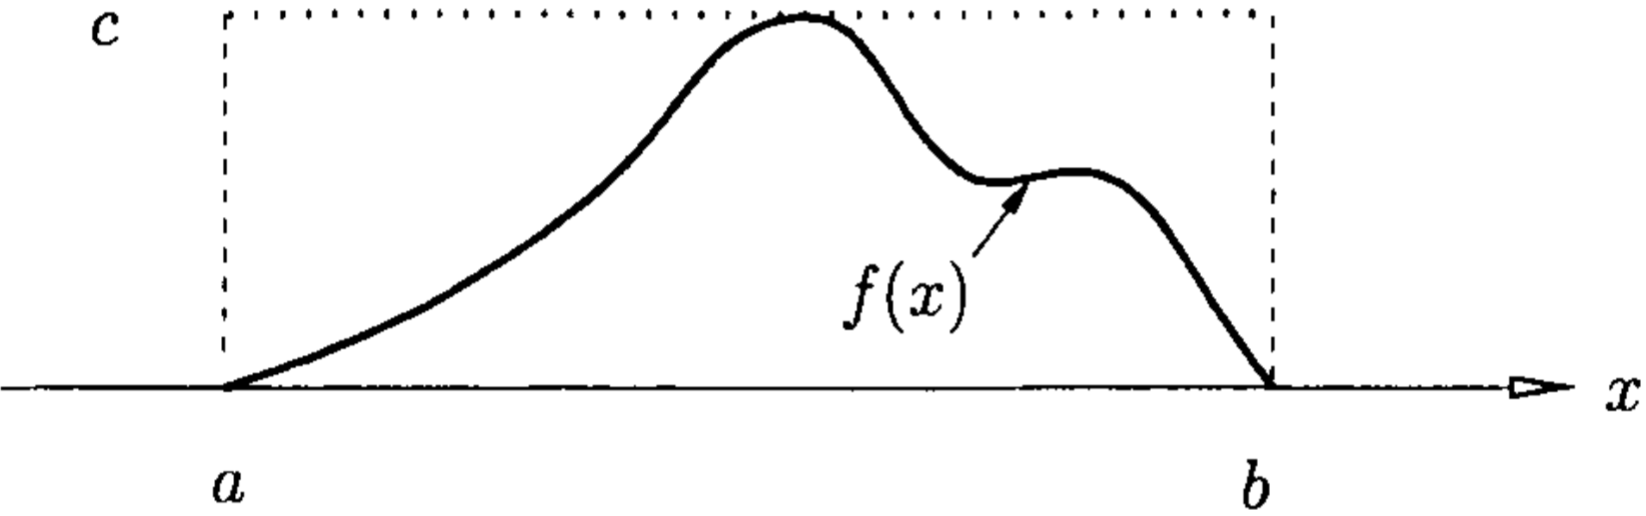
\includegraphics[width=0.65\textwidth]{graphics/gi/mc-6}
	\caption{The acceptance-rejection method.}
	\label{f:rejection-idea}
\end{figure}

In this case, generating a random variable $Z\sim f$ is straightforward, and it can be done using the following acceptance-rejection steps:

\begin{enumerate}
	\item Generate $X\sim U(a,b)$.
	\item Generate $Y\sim U(0,c)$ independently of $X$ ($c$ is the maximum of $f$). 
	\item If $Y\leq f(X)$, return $Z=X$. Otherwise, return to step 1.
\end{enumerate}

It is important to note that each generated vector $(X,Y)$ is uniformly distributed over the rectangle $[a,b]\times [0,c]$. Therefore, the accepted pair $(X,Y)$ is uniformly distributed under the graph $f$. This implies that the distribution of the accepted values of $X$ has the desired PDF $f$.

\begin{figure}
\sidecaption
	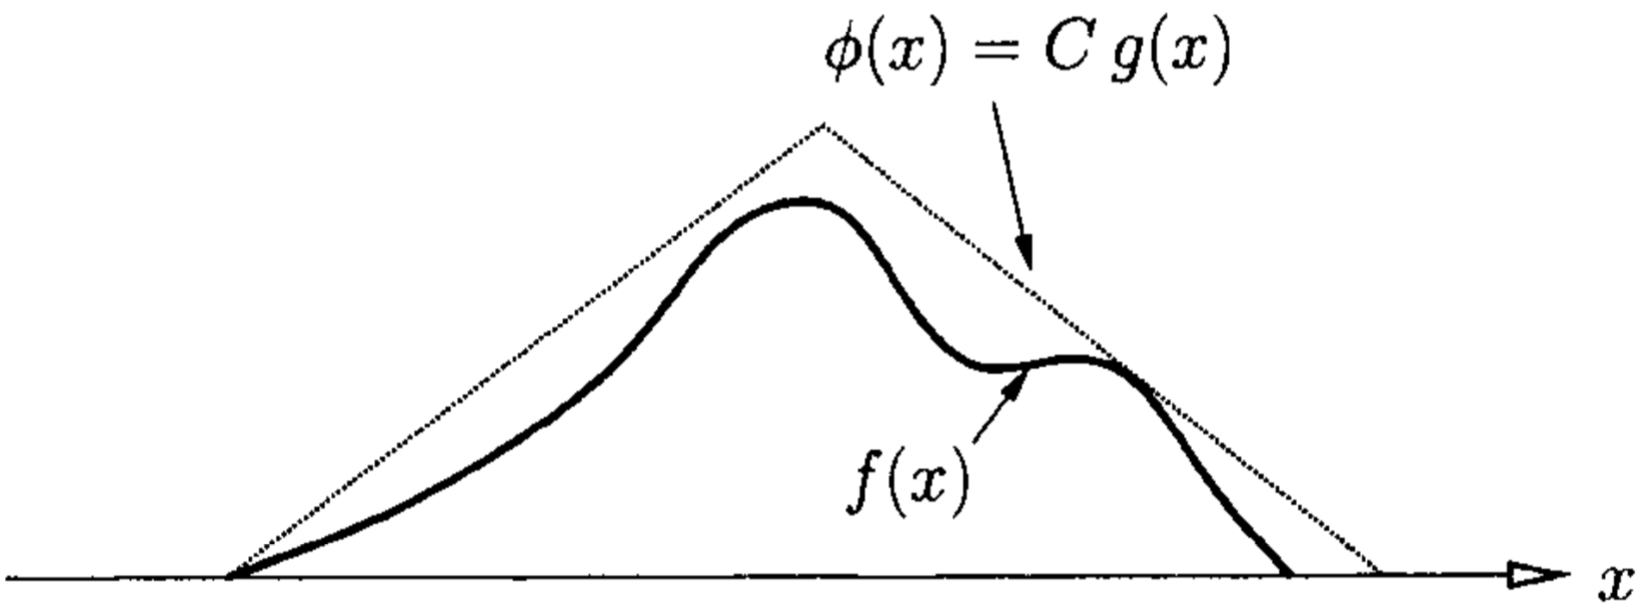
\includegraphics[width=0.65\textwidth]{graphics/gi/mc-7}
	\caption{The acceptance-rejection method with a majorizing function $\phi$.}
	\label{f:rejection-generalized}
\end{figure}

The disadvantage of this method is that it has low efficiency, that is, many values are rejected before one is accepted. In practice, it is usually use a $\phi (x=)Cg(x)$ (instead of $c$), which tightly bounds to $f(x)$ and is easy to generate random variables, to majorize $f$. We call $g(x)$ the \textit{proposal} PDF, see figure \ref{f:rejection-generalized}. The acceptance-rejection algorithm can be written as follows:

\begin{enumerate}
	\item Generate $X$ from $g(x)$.
	\item Generate $Y\sim U(0,Cg(X))$.
	\item If $Y\leq f(X)$, return $Z=X$. Otherwise, return step 1. 
\end{enumerate}


\subsection{Transformation of Random Variables}\label{sec:Transformation-of-Random-Variables}
In describing the inversion method, we introduced a technique that generates samples according to some distribution by transforming canonical uniform random variables in a particular manner. Here, we will investigate the more general question of which distribution results when we transform samples from an arbitrary distribution to some other distribution with a function $f$.

Suppose that $X$ is a random variable with cumulative distribution $F_X(x)$ and PDF $f_X(x)=\frac{dF_X}{dx}$, and that the random variable $Y=y(X)$ is a continuous nondecreasing function of $x$ as in \ref{f:transforming-function}(a). What is $F_Y(y)$? The variable $X$ and the function $y(X)$ map into each other:

\begin{equation}
	y(X)\leq y(x), \text{ if } X\leq x
\end{equation}

so the probabilities become

\begin{equation}
	P\{y(X)=Y\leq y(x)\}=P\{X\leq x\}
\end{equation}

\begin{figure}
	\begin{subfigure}[b]{.48\textwidth}
		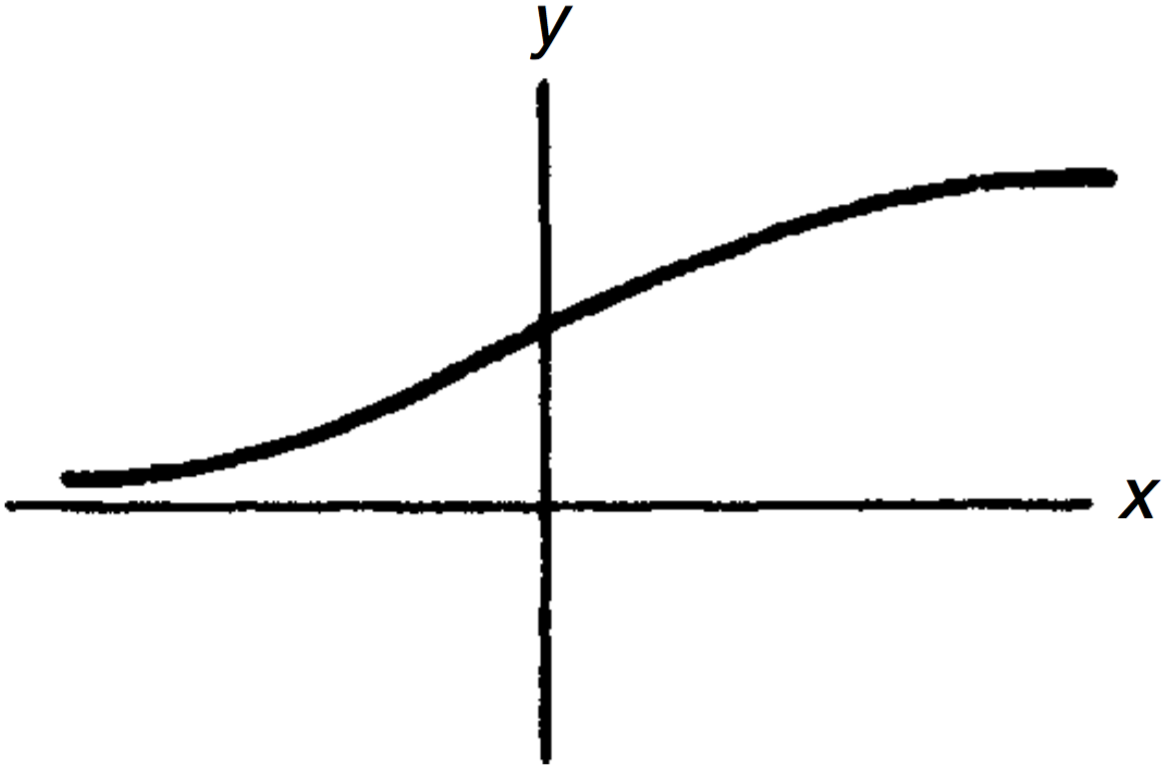
\includegraphics[width=1.\textwidth]{graphics/gi/mc-8}
		\caption{nondecreasing}
	\end{subfigure}
	\begin{subfigure}[b]{.48\textwidth}
		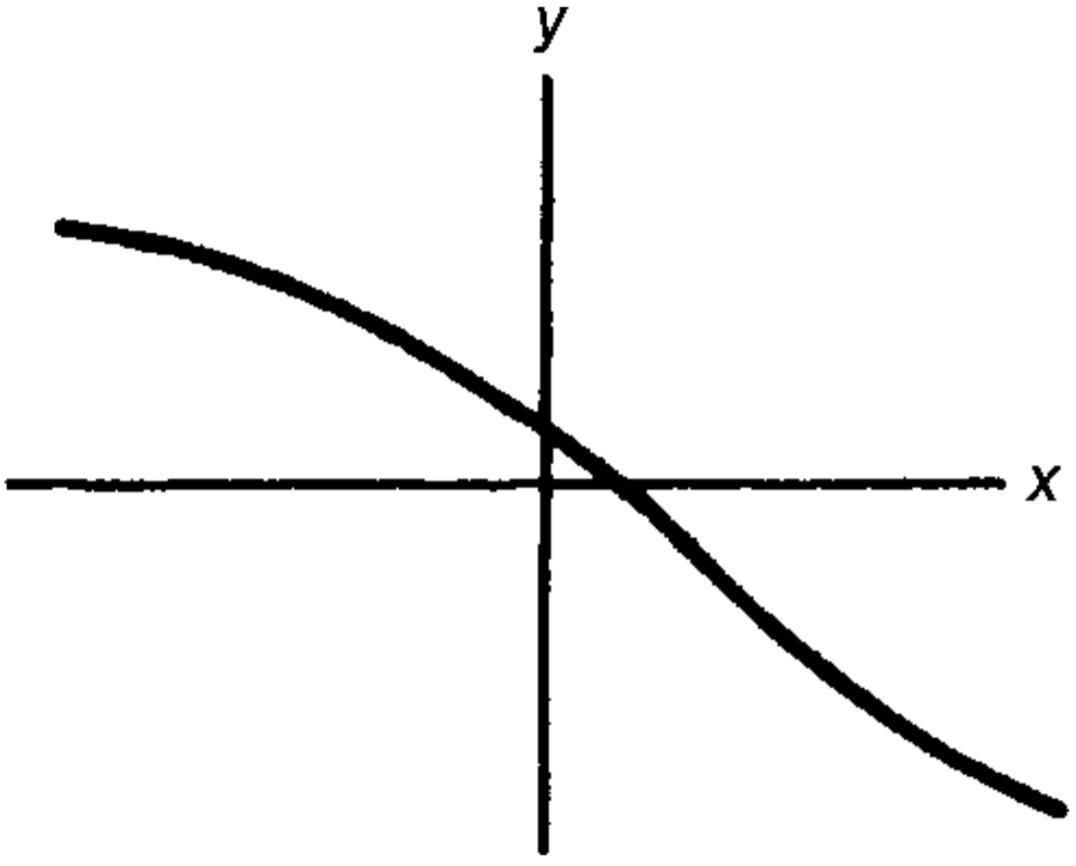
\includegraphics[width=1.\textwidth]{graphics/gi/mc-9}
		\caption{nondecreasing}
	\end{subfigure}
	\caption{$y$ is a continuous a: nondecreasing/ b: nonincreasing function of $x$}
	\label{f:transforming-function}
\end{figure}

or
\begin{equation}\label{e:label123}
	F_Y(y)=F_X(x)
\end{equation}

The relationship between the probability distribution functions may be determined by differentiating equation \ref{e:label123}:

\begin{equation}
	f_Y(y)\frac{dy}{dx}=f_X(x)
\end{equation}


Suppose that $y(X)$ is a nonincreasing function of $X$ (see figure \ref{f:transforming-function}(b)), then:

\begin{equation}
	f_Y(y)\frac{dy}{dx}=-f_X(x)
\end{equation} 

The relationship between the PDF's of X and Y for both cases can be combined in one equation as

\begin{equation}
	f_Y(y)=|\frac{dy}{dx}|^{-1}f_X(x)
\end{equation}

reflecting the fact that all the values of $X$ in $dx$ map into values of $Y$ in $dy$, see figure \ref{f:pdf-map}.

\begin{figure}
\sidecaption
	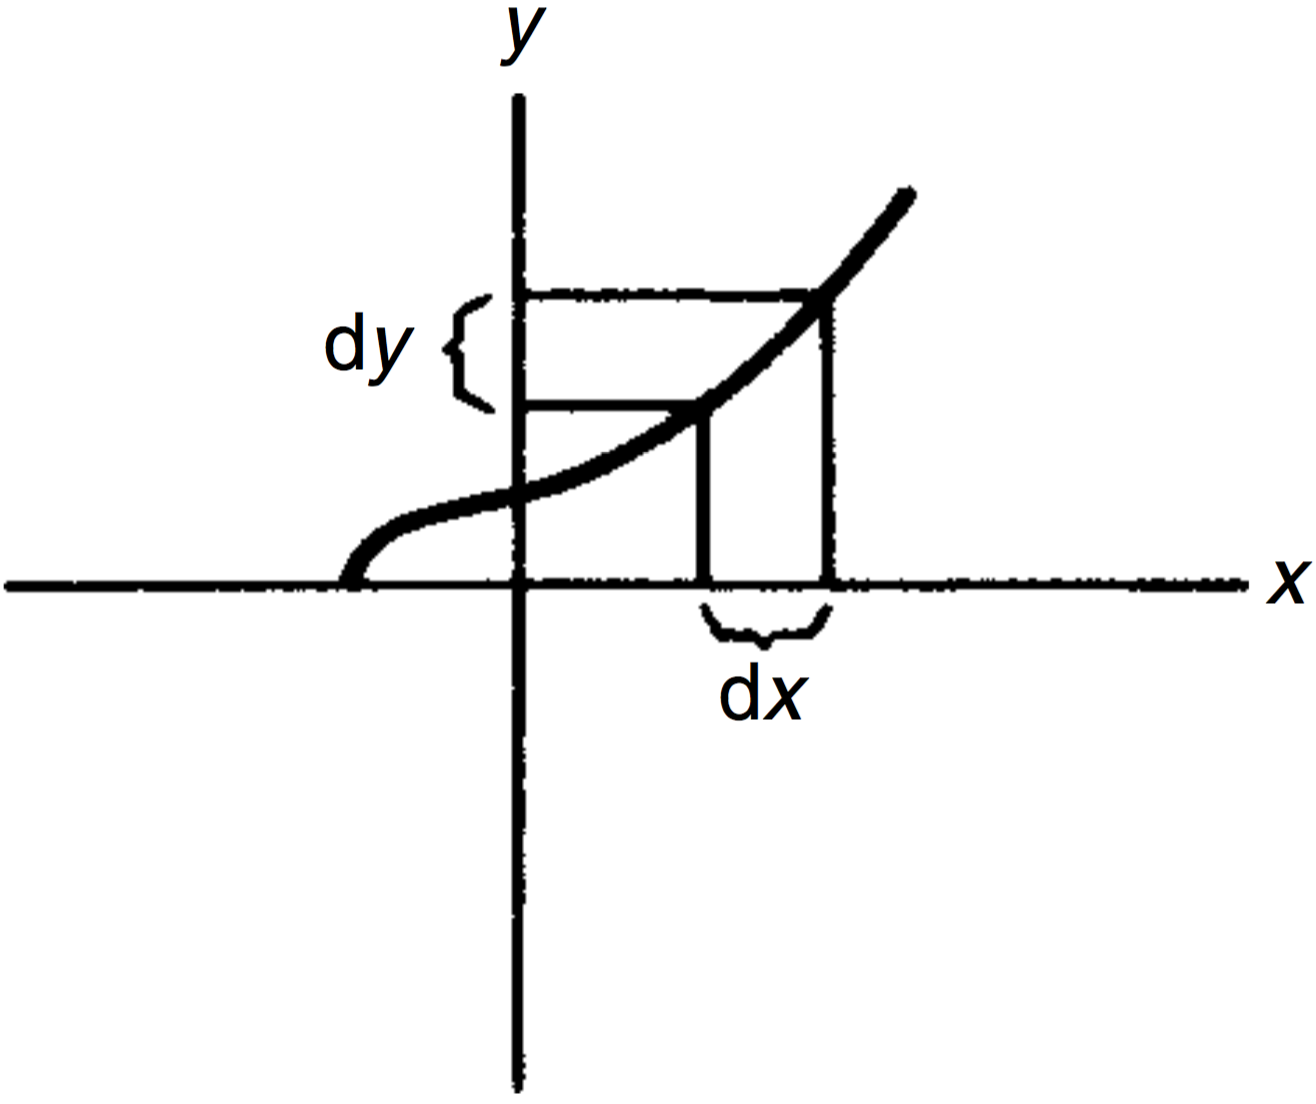
\includegraphics[width=0.65\textwidth]{graphics/gi/mc-10}
	\caption{Values of $X$ in $dx$ map into values of $Y$ in $dy$.}
	\label{f:pdf-map}
\end{figure}

\subsubsection{Transformation in Multiple Dimensions}
In the general $n$-dimensional case, a similar derivation gives the analogous relationship between different densities. We will not show the derivation here; it follows the same form as the one-dimensional case. Suppose we have an $n-$dimensional random variable $X$ with density function $p_x(x)$. Now let $Y = T (X)$, where $T$ is a bijection. In this case, the densities are related by

\begin{equation}
	p_y(y)=p_y(T(x))=\frac{p_x(x)}{|J_T(x)|}	
\end{equation}

where $|J_T|$ is the absolute value of the determinant of $T$'s Jacobian matrix, which is

\begin{equation}
	\begin{pmatrix}
  	\partial{T_1}/\partial{x_1} & \cdots & \partial{T_1}/\partial{x_n} \\
  	\vdots                      & \ddots & \vdots \\
  	\partial{T_n}/\partial{x_1} & \cdots & \partial{T_n}/\partial{x_n}
	\end{pmatrix}
\end{equation}

where $T_i$ are defined by $T(x) = (T_1(x), . . . , T_n(x))$.



\section{Variance Reduction}\label{sec:Variance-Reduction}
We've known how to calculate integration using Monte Carlo method. Basically, we first using the aforementioned sampling methods (such as inversion or rejection method) to draw $N$ random variables according to some probability distribution function $p(x)$, then we evaluate every sample's value by $\frac{f(x)}{p(x)}$, and finally we average these values to get the estimate of the integral of $f(x)$. 

Since it is a stochastic process, variance exists. Designing efficient estimators is a major area of research in Monte Carlo literature. This section we will discuss some techniques that can reduce variance.




\subsection{Importance Sampling}
Importance sampling is a technique that can reduce variance by choosing samples from a distribution $p(x)$, which has a \textit{similar shape} as the function $f(x)$ being integrated. Intuitively, importance sampling attempts to place more samples where the contribution of the integrand is high, or "importance".

Given a PDF $p(x)$ defined over the integration domain $D$, and samples $x_i$ generated according to the PDF, the value of the integral $I$ can be estimated by generating $N$ sample points and computing the weighted mean:

\begin{equation}
	\langle I\rangle=\frac{1}{N}\sum_{i=1}^{N}\frac{f(x_i)}{p(x_x)}
\end{equation}

A \textit{perfect estimator} would have the variance be zero. The optimal $p(x)$ for the perfect estimator can be derived from:

\begin{equation}
	0=\sigma^2=\frac{1}{N}\int(\frac{f(x)}{p(x)}-I)^2p(x)dx
\end{equation}

because $p(x)$ is nonzero, so:

\begin{equation}
	p(x)=\frac{|f(x)|}{I}
\end{equation}

If we use this $p(x)$, the variance will be exactly zero. However, this optimal $p(x)$ requires us to know the value of $I$, which is exactly the integral we want to compute to begin with. Clearly, finding the optimal $p(x)$ is impossible. However, by choosing a PDF that is similar to $f(x)$, we can make the variance arbitrary low.

\begin{figure}\label{f:iimportance-figure}
	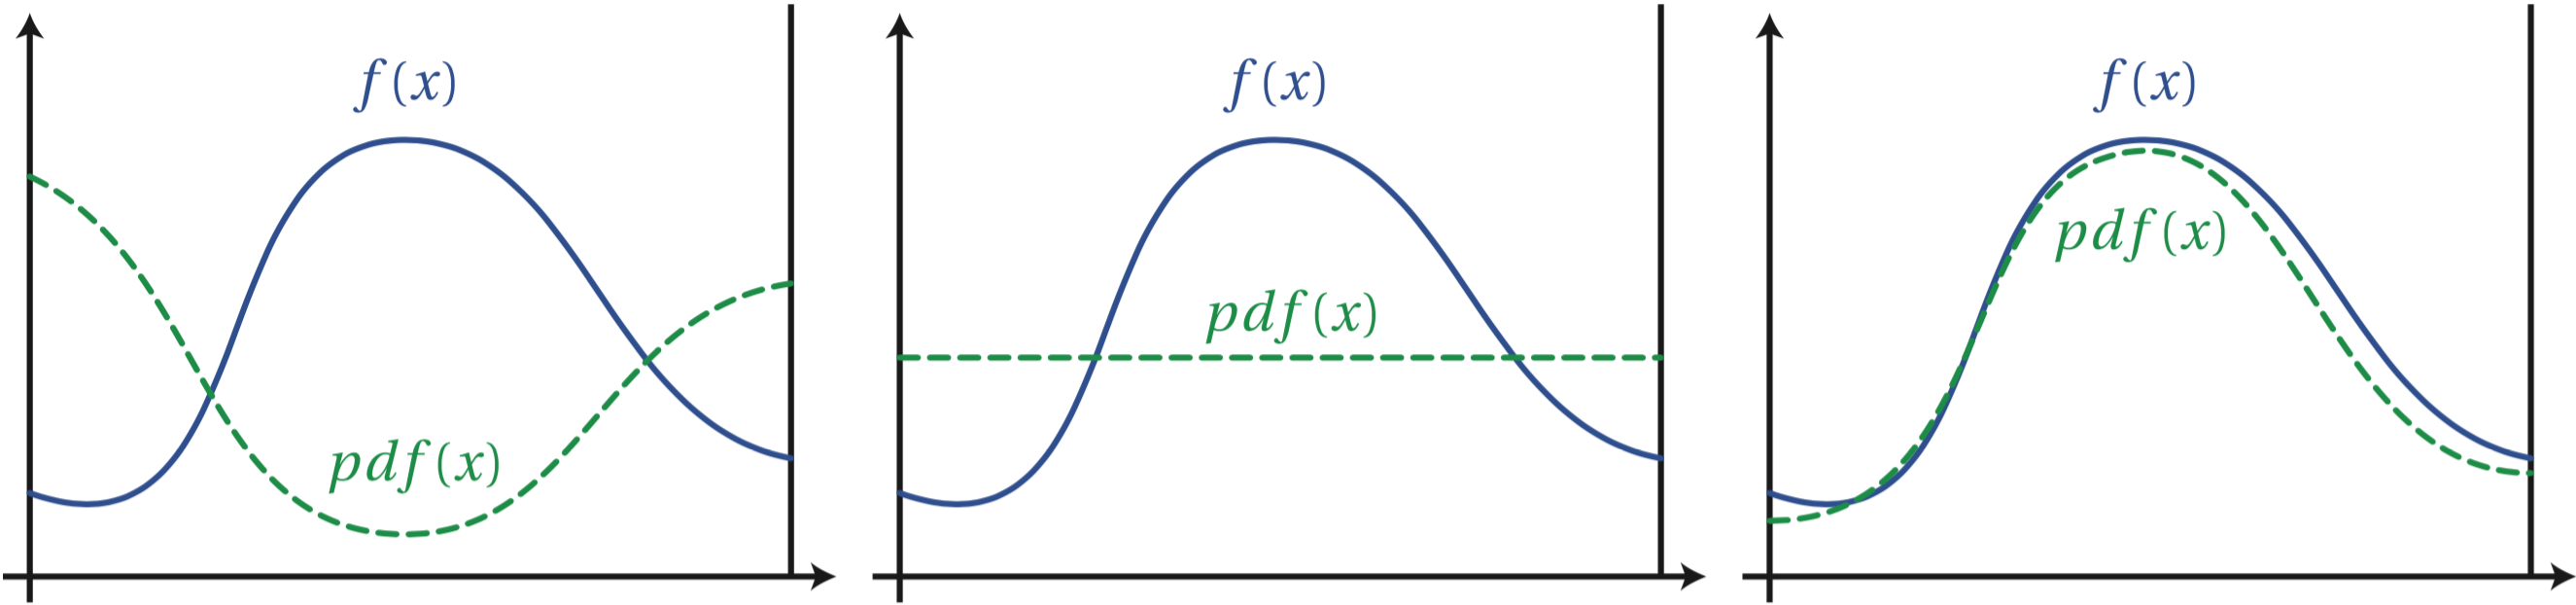
\includegraphics[width=0.65\textwidth]{graphics/gi/mc-11}
	\caption{Comparison of three probability density functions.}
\end{figure}

Figure \ref{f:iimportance-figure} shows three different probability functions, the variance of the estimator on the left-hand side will be large than the variance of the estimator shown on the right-hand side; and using the PDF on the left would significantly increase variance over simple uniform sampling in the center. 




\subsection{Multiple Importance Sampling}
In real situation, the functions that we need to integrate in computer graphics are often ill-behaved. They are almost always discontinuous, and often have singularities or very large values over small portions of their domain. It's hard to find a "similar" distribution to this functions.

For example, consider the problems of evaluating direct lighting integrals of the form which we have seen before:

\begin{equation}
	L_o(\mathbf{p},\mathbf{v})=\int_{\Omega}f(\mathbf{l},\mathbf{v})\otimes L_i(\mathbf{p},\mathbf{l})cos\theta_i d\omega_i
\end{equation}

If we were to perform importance sampling to estimate this integral according to distributions based on either $L_i$ of $f_r$, one of these two will often perform poorly.

Consider a near-mirror BRDF illuminated by an area light where $L_i$'s distribution is used to draw samples. Because the BRDF is almost a mirror, the value of the integrand will be close to zero at all $\omega_i$ directions except those around the perfect specular reflection direction. This means that almost all of the directions sampled by $L_i$ will have zero contribution, and variance will be quite high. While sampling from the BRDF's distribution would be a much better approach to this particular case, for diffuse or glossy BRDFs and small light sources, sampling from the BRDF's distribution can similarly lead to much higher variance than sampling from the light's distribution.

\begin{figure}\label{f:mis}
	\begin{subfigure}[b]{0.328\textwidth}
		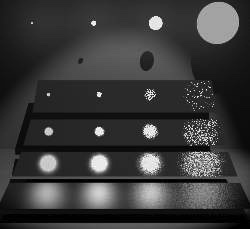
\includegraphics[width=1.\textwidth]{graphics/gi/mis-1}
		\caption{Sampling the light source}
	\end{subfigure}
	\begin{subfigure}[b]{0.328\textwidth}
		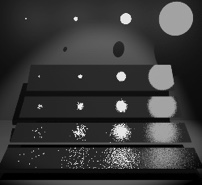
\includegraphics[width=1.\textwidth]{graphics/gi/mis-2}
		\caption{Sampling the BRDF}
	\end{subfigure}
	\begin{subfigure}[b]{0.328\textwidth}
		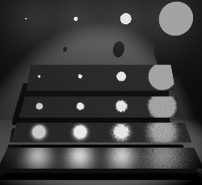
\includegraphics[width=1.\textwidth]{graphics/gi/mis-3}
		\caption{MIS}
	\end{subfigure}
	\caption{Sampling of glossy highlights from area light sources. There are four spherical light sources of varying radance and color, plus a spotlight overhead. All spherical light sources emit the same total power. There are also four shiny rectangular plates of varying surface roughness, each one tilted so that we see the reflected light sources.}
\end{figure}

Because of this, we often need more than one sampling technique to estimate an integral with low variance. Normally this is accomplished by explicitly partitioning the domain of integration into serval regions, and designing a sampling technique for each region. 

\textit{Multiple importance sampling} (MIS) addresses this problems with a simple and easy-to-implement technique. MIS provides a strategies that compute \textit{weighted combination} of samples from serval distributions. This approach has three steps according to the original paper\cite[28mm]{a:OptimallyCombiningSamplingTechniquesforMonteCarloRendering}:

\begin{itemize}
	\item First, we design a set of importance sampling distributions $p_1,...,p_n$. For each region where $f$ has the potenntial to be large, we try to construct a sampling distribution that approximates $f$ well over that portion of the domain. An excellent source of these distributions is the situation where $f$ is a product of serval unrelated functions, and each $p_i$ is proportional to the product of a subset of these.
	\item Next, we determine how many samples to take from each $p_i$. We assume this is fixed in advance, based on knowledge of $f$ and $p_i$.
	\item Finally, the integral is estimated as a weighted combination of all the sample values. 
\end{itemize}

Consider unbiased estimators that allow samples to be weighted differently, depending on which underlying distribution $p_i$ they were chosen from. Each estimator is parameterized by a set of \textit{weighting functions} $\omega_1,...,\omega_n$, where $\omega_i(x)$ gives the weight associated with a sample $x$ drawn from $p_i$. The \textit{combined estimator} is given by:

\begin{equation}\label{e:combined-estimator}
	\langle I \rangle=\sum_{i=1}^{n}\frac{1}{n_i}\sum_{j=1}^{n_i}\omega_i(X_{x,j})\frac{f(X_{i,j})}{p_i(X_{i,j})}
\end{equation}

where the $X_{x,j}$ are independent samples from distribution $p_i$. For this estimator to be unbiased, the $\omega_i$ must satisfy $\omega_i(x)=0$ whenever $p_i(x)=0$, and $\sum_{i}\omega_i(x)=1$ whenever $f(x)\neq 0$. We can then show:

\begin{equation}
	E[\langle I\rangle]=\sum_{i=1}^{n}\frac{1}{n_i}n_i\int_{\Omega}\frac{\omega_i(x)f(x)}{p_i(x)}p_i(x)d\mu (x)=\int_{\Omega}f(x)d\mu (x)
\end{equation}

Based on this standard multi-sample model, different weighting functions can be chosen to minimize the variance.


\subsubsection{The Balance Heuristic}
Consider the weighting functions:

\begin{equation}
	\hat{\omega}_i(x)=\frac{c_ip_i(x)}{\sum_j c_jp_j(x)}
\end{equation}

where $c_i$ is the relative number of samples taken from $p_i$, where $\sum_i c_i=1$ and the $c_i$ are fixed in advance. These $\hat{\omega}_i$ have the unique property that the sample value $\frac{\hat{\omega}_i(x)f(x)}{n_ip_i(x)}$ from \ref{e:combined-estimator} does not depend on $i$. Because the sample value at a particular $x$ is the same for all underlying distributions, we call this strategy the \textit{balance heuristic}.

Substituting $\hat{\omega}_i$ into equation \ref{e:combined-estimator}, we get the standard estimator:

\begin{equation}
	\langle I\rangle=\frac{1}{N}\sum_{i=1}^{n}\sum_{j=1}^{n_i}\frac{f(X_{i,j})}{\bar{p}(X_{i,j})}
\end{equation} 

where:

\begin{equation}
	\bar{p}(x)=\sum_{i=1}^{n}c_ip_i(x)
\end{equation}

which is called the \textit{combined sample distribution}. Here $n_i=c_i N$ independent samples $X_{i,j}$ are taken from distribution $p_i$, for a total of $N$ samples.

This is the key ideas of balance heuristic. And this is the natural way to combine multiple distributions. We use the single $\bar{p}(x)$, which does not depend on $i$, to represent the combinations. More precisely, $\bar{p}(x)$ is the distribution of a random variable $X$ which is equal to each $X_{i,j}$ with probability $1/N$.

Besides the standard form, serval different strategies for weighting functions have been proposed. For interested readers, please goto: \cite{a:Safeandeffectiveimportancesampling}, \cite[3mm]{a:AdaptiveMultipleImportanceSampling}, \cite[3mm]{a:ANADAPTIVEPOPULATIONIMPORTANCESAMPLER} and \cite[3mm]{a:EfficientMultipleImportanceSamplingEstimators}.



\subsection{Careful Sample Placement}
Importance sampling places more samples where the function is deemed more importance. The problem with this is that it does not eliminate sample "\textit{clumping}", as the PDF only dictates the expected number, not the actual number, of samples in any given region.

A classic and effective family of techniques based on careful placement of samples in order to capture "importance" features of the integrand. These techniques are usually complementary to techniques like importance sampling. This section is going to discuss this kind of techniques which try to minimize clumping to reduce variance.


\subsubsection{Stratified Sampling}
Stratified sampling works by subdividing the domain $\Omega$ into serval non-overlapping regions $\Omega_1,...,\Omega_n$ such that:

\begin{equation}
	\bigcup_{i=1}^{n}\Omega_i=\Omega
\end{equation}

Each region $\Omega_i$ is called a \textit{stratum}. A fixed number of samples $n_i$ is then taken within each $\Omega_i$, according to some given density function $p_i$.

Within a single stratum $\Omega_i$, the Monte Carlo estimator is:

\begin{equation}
	F_i=\frac{1}{n_i}\sum_{j=1}^{n_i}\frac{f(X_{i,j})}{p_i(X_{i,j})}
\end{equation} 

where $X_{i,j}$ is the $j$th sample drawn from density $p_i$. The overall estimate is :

\begin{equation}
	F=\sum_{i=1}^{n}v_iF_i
\end{equation}

where $v_i$ is the fractional volume of stratum $i$ ($v_i\in(0,1]$). The variance of this estimator is 

\begin{figure}
\begin{center}
	\begin{subfigure}[b]{0.48\textwidth}
		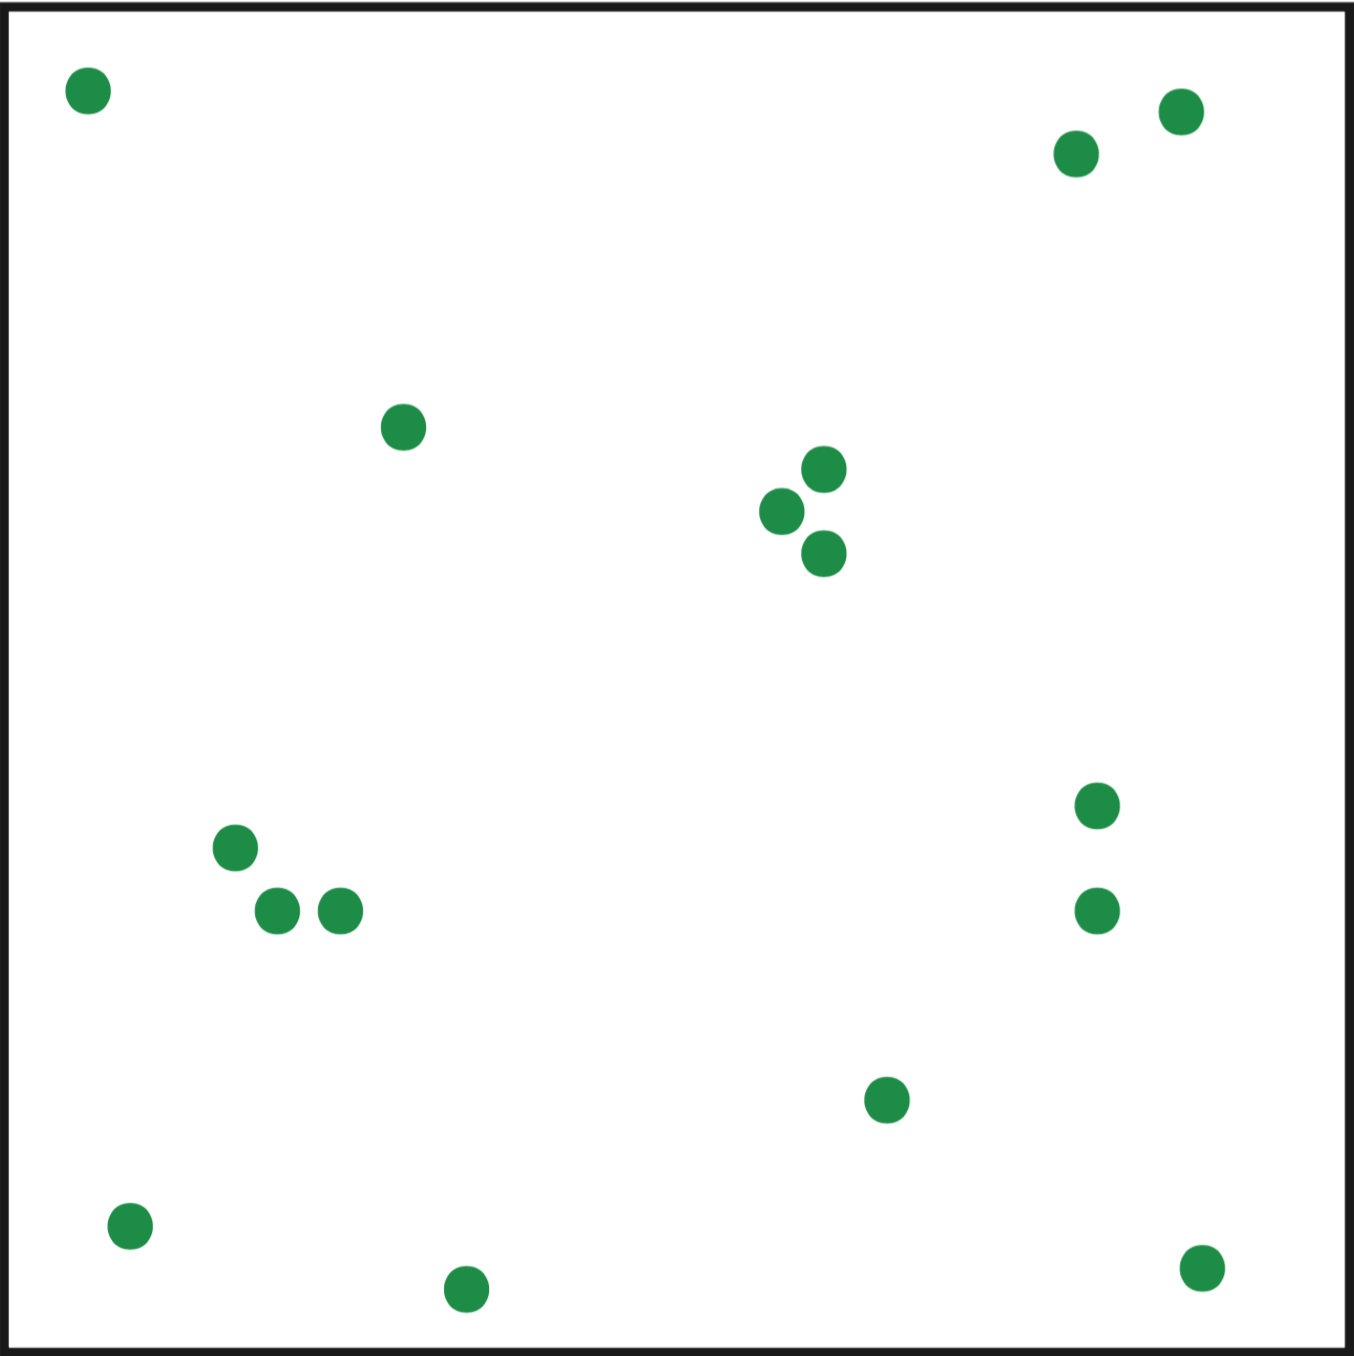
\includegraphics[width=1.\textwidth]{graphics/gi/mc-12-1}
		\caption{Random}
	\end{subfigure}
	\begin{subfigure}[b]{0.48\textwidth}
		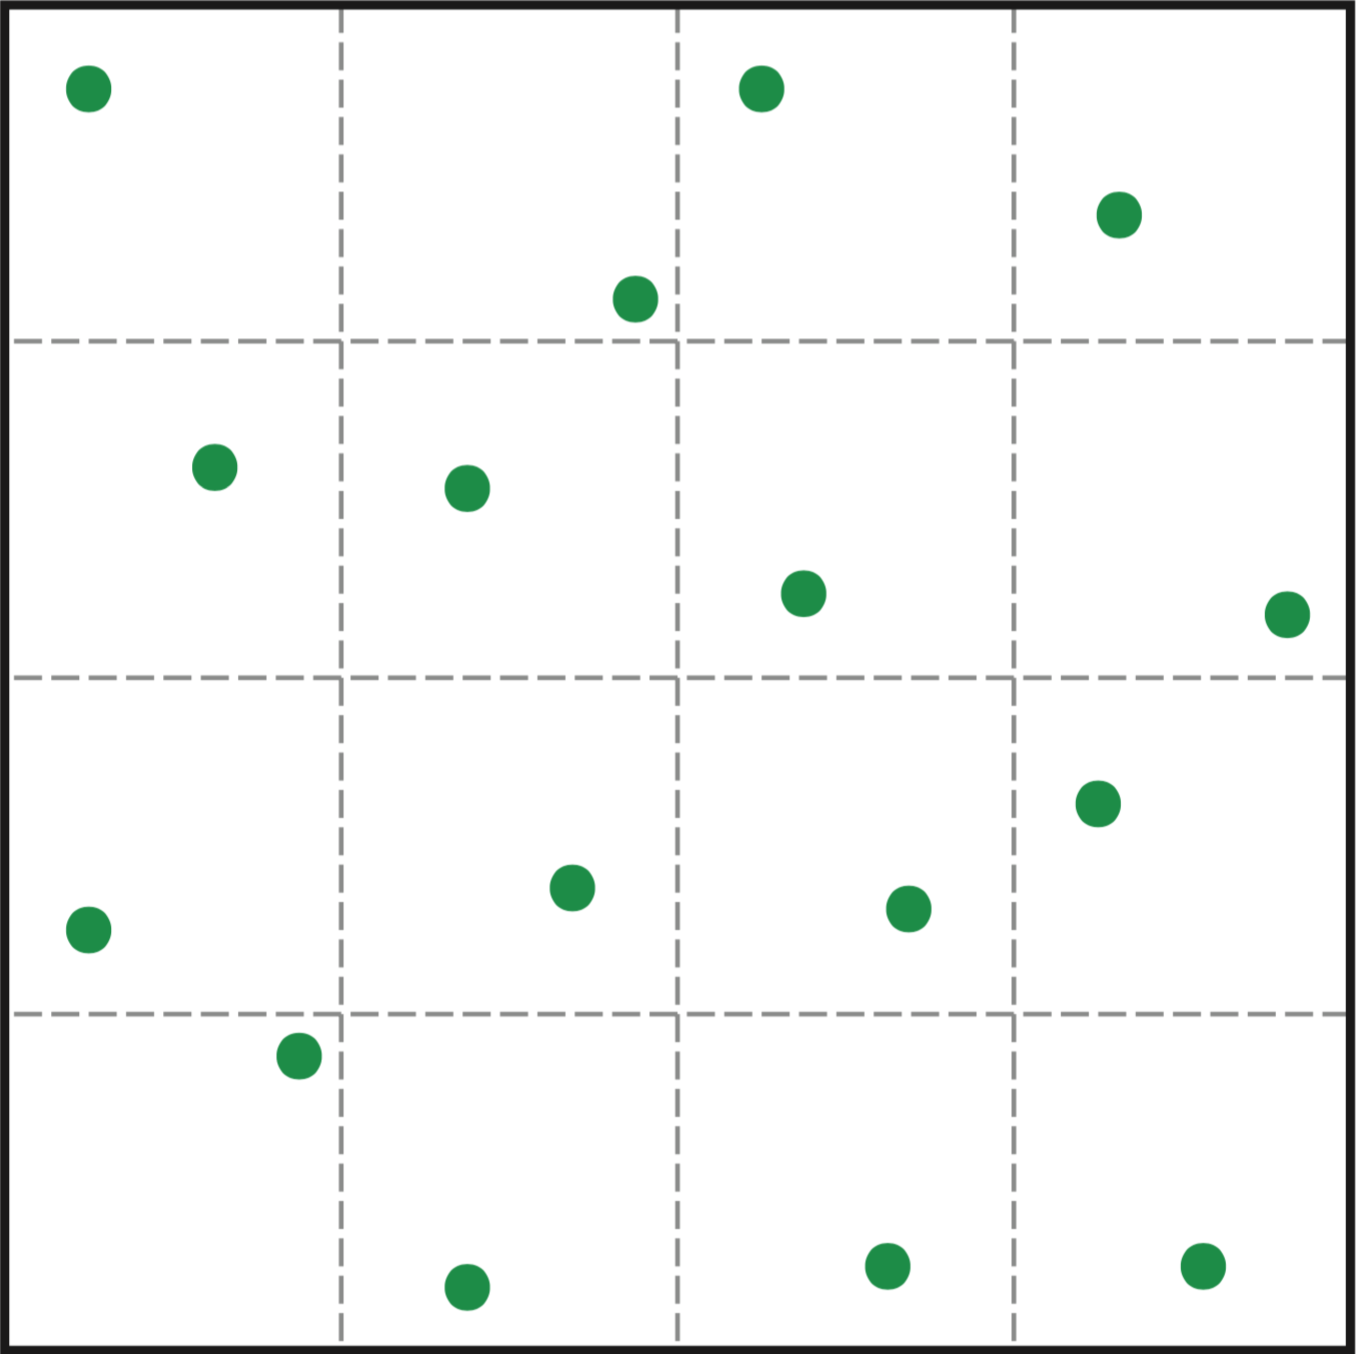
\includegraphics[width=1.\textwidth]{graphics/gi/mc-12-2}
		\caption{Stratified}
	\end{subfigure}
\end{center}
	\caption{Comparison of random and stratified sampling approaches each using 16 samples. Purely random sampling (a) can suffer from clumping, which increases variance by undersampling other regions of the integrand. }
	\label{f:placement}
\end{figure}


\begin{equation}
	V[F]=\sum_{i=1}^{n}\frac{v_{i}^2 \sigma_{i}^2}{n_i}
\end{equation}

where $\sigma_{i}^2=V[f(X_{i,j})]$ denotes the variance of $f$ within $\Omega_i$.

To compare this against unstratified sampling, suppose that $n_i=v_iN$, where $N$ is the total number of samples taken. The above equation then simplifies to:

\begin{equation}
	V[F]=\frac{1}{N}\sum_{i=1}^{n}v_{i} \sigma_{i}^2
\end{equation}

On the other hand, the variance of the corresponding unstratified estimator is (See page 51 of \cite[5mm]{a:RobustMonteCarloMethodsforLightTransportSimulation} for a derivation of this result):

\begin{equation}
	V[F]=\frac{1}{N}\Bigg[ \sum_{i=1}^{n}v_{i} \sigma_{i}^2 +\sum_{i=1}^{n}v_i(\mu_i-I)^2   \Bigg]
\end{equation}

where $\mu_i$ is the mean value of $f$ in region $\Omega_i$, and $I$ the mean value of $f$ over the whole domain. Since the right-hand sum is always non-negative, stratified sampling can never increase variance, see figure \ref{f:placement}.

The main problem of Stratified sampling is that it is not helpful for high dimension integral. In general, $N^d$ strata would need to be created for a $d$ dimensional domain. For this problem, some variant have been proposed. The $N$-rooks algorithm keeps the number of samples fixed (irrespective of dimensionality). Quasi-Monte Carlo sampling uses nonrandom samples to avoid clumping.




\begin{figure}
\sidecaption
	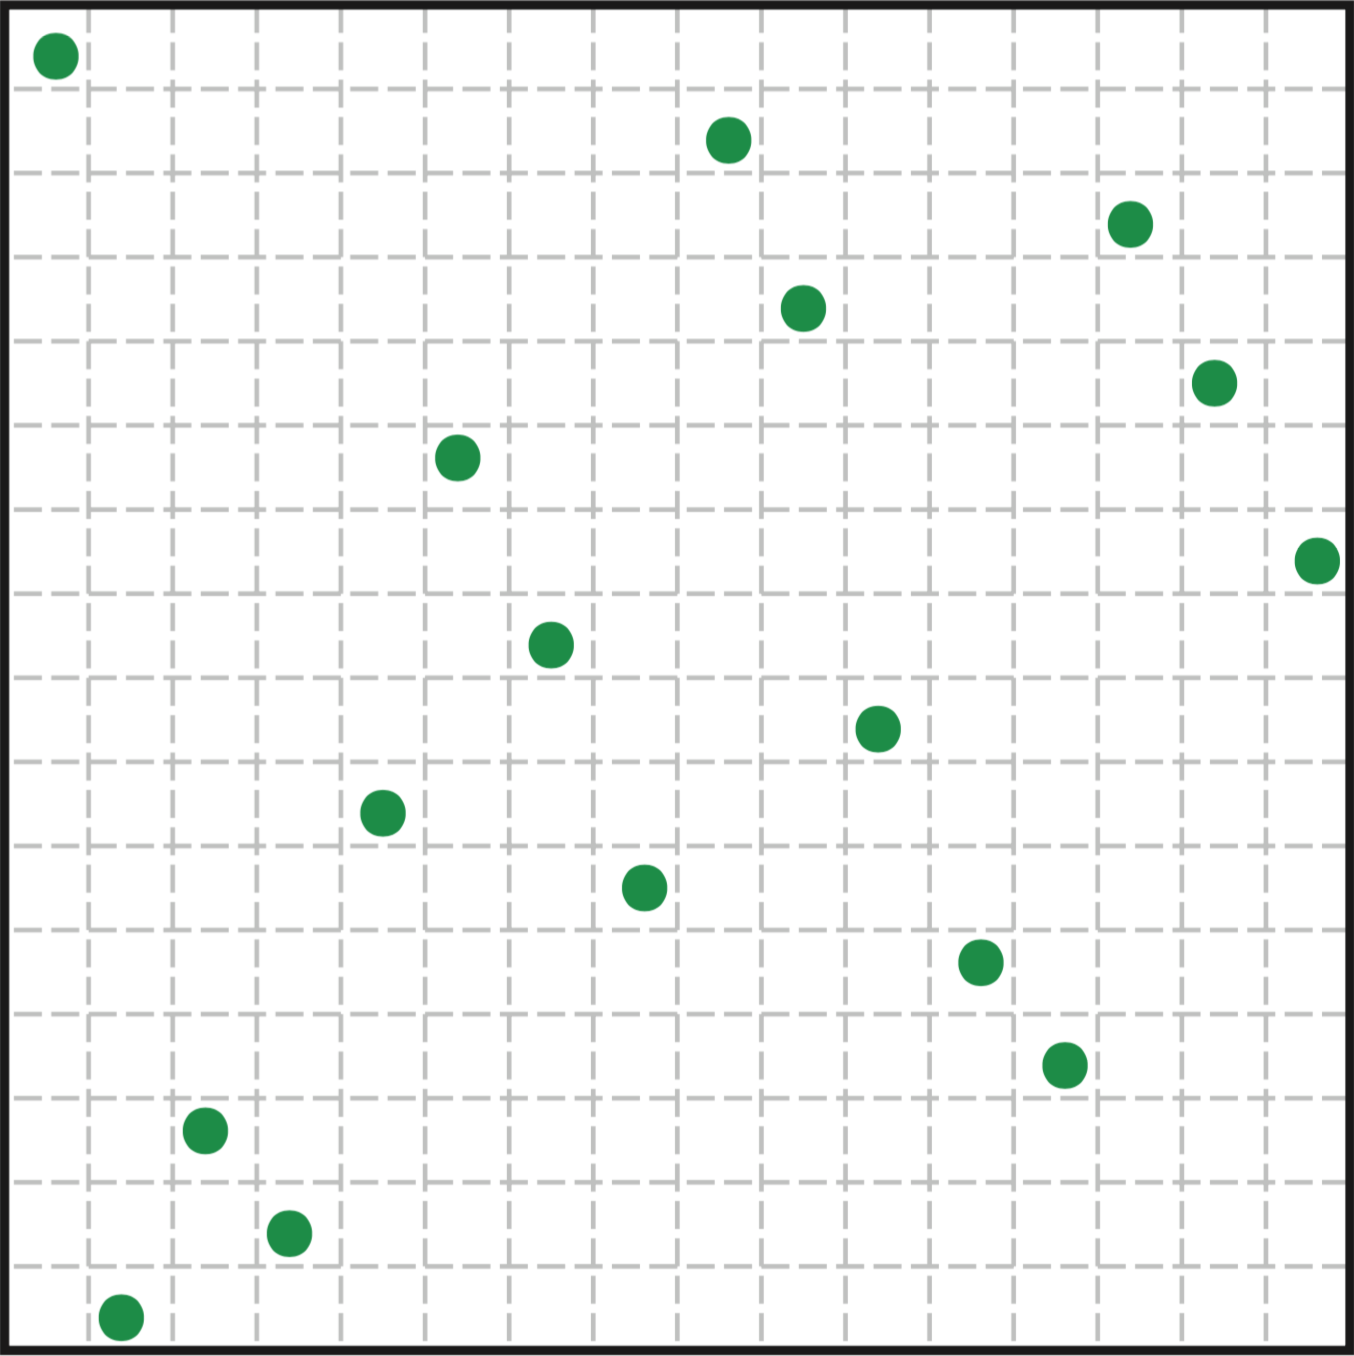
\includegraphics[width=0.6\textwidth]{graphics/gi/mc-12-3}
	\caption{$N$-rooks sampling, in two dimensions, this means that no row or column has more than one sample.}
	\label{f:n-rooks}
\end{figure}





\subsubsection{N-Rooks or Latin Hypercube Algorithm}
Consider, for example, a two-dimensional function, stratification of both dimensions would require $N^2$ strata with one sample per stratum. The $N$-rooks algorithm addresses this by distributing $N$ samples evenly among the strata. That is each row and column of a grid will have one sample, see figure \ref{f:n-rooks}. For details, see Shirley's Ph.D. thesis \cite[-5mm]{a:PhysicallyBasedLightingCalculationsForComputerGraphics}. 


\subsubsection{Quasi-Monte Carlo}\label{sec:quasi-monte-carlo}

\footnote{\url{https://en.wikipedia.org/wiki/Quasi-Monte_Carlo_method}}





